%%% Document Formatting
\documentclass[12pt,fleqn]{article}
\usepackage[a4paper,
            bindingoffset=0.2in,
            left=0.75in,
            right=0.75in,
            top=0.8in,
            bottom=0.8in,
            footskip=.25in]{geometry}
\setlength\parindent{10pt} % No indent

%%% Imports
% Mathematics
\usepackage{amsmath} % Math formatting
\numberwithin{equation}{section} % Number equation per section
\DeclareMathOperator{\Tr}{Tr}


\newtheorem{theorem}{Theorem}
\newtheorem{definition}{Definition}
\newtheorem{proof}{Proof}
\newtheorem{lemma}{Lemma}
\newtheorem{example}{Example}

\usepackage{amsmath}
\usepackage{amsfonts} % Math fonts
\usepackage{amssymb} % Math symbols
\usepackage{mathtools} % Math etc.
\usepackage{slashed} % Dirac slash notation
\usepackage{cancel} % Cancels to zero
\usepackage{empheq}
\usepackage{breqn}

\newcommand{\expect}{\mathbb{E}}


% Visualization
\usepackage{graphicx} % for including images
\graphicspath{ {} } % Path to graphics folder
\usepackage{tikz}



%%% Formating
\usepackage{hyperref} % Hyperlinks
\hypersetup{
    colorlinks=true,
    linkcolor=blue,
    filecolor=magenta,      
    urlcolor=cyan,
    pdftitle={Overleaf Example},
    pdfpagemode=FullScreen,
    }
\urlstyle{same}

\usepackage{mdframed} % Framed Enviroments
\newmdenv[ 
  topline=false,
  bottomline=false,
  skipabove=\topsep,
  skipbelow=\topsep
]{sidework} %% Side-work

\usepackage{lipsum} % Lorem Ipsum example text

%%%%% ------------------ %%%%%
%%% Title
\title{Lectures Notes from Beg Rohu 2025}
\author{Clark Miyamoto (cm6627@nyu.edu)}
\date{\today}
\begin{document}

\maketitle
\begin{abstract}
	Hello....
\end{abstract}

\tableofcontents
\newpage

\part{Mallat: Score Based Diffusion \& Renormalization Group Flow}
\section{Overview}
We'll be going from score-diffusion and eventually make our way to the renormalization group.\\
\\
The setup is you're given a set of input data $\{x_i : x_i \in \mathbb R^d\}_{i \leq n}$ which (we believe) to be sampled from a distribution $p(x)$. Your objective is to reconstruct this probability distribution.\\
\\
Doing this problem in the physics context, the canonical example will be attempting to recreate samples from a Ising / $\phi^4$ model. Some more advanced problems are turbulence, cosmology, metrology, and climatology. Apart from physics, you can also generate new image (i.e. conditional generation), and use it to solve inverse problems.\\
\\
As you start to think more about this problem, it might seem hopeless to learn $p(x)$. This is because the problem suffers from the \textbf{curse of dimensionality}. A crude way to calculate this is to first assume $p(x)$ is Lipschifts
\begin{definition}
	[Lipschifts] That is $| p(x) - p(x') | \leq K \underbrace{|| x- x' ||}_{\epsilon \in [0,1]^d}$
\end{definition}
This means you'll need $\sim C \epsilon^{-d}$ amount of data... You can see you're screwed.\\
\\
We can start to tackle this problem by making a key assumption, factorize the distribution
\begin{align}
	p(x) = \prod_k p_k(x) \implies \log p(x) = \sum_k \log p_k(x)
\end{align}
Two problems now emerge
\begin{enumerate}
	\item How do we choosing this factorization?
	\item How do we prevent it from just simply memorizing a distribution?
\end{enumerate} 
The first method is to assume $p(x)$ is a empirical distribution, by this I mean $p(x) = \frac{1}{n} \sum_{i=1}^n  \delta_{x_i}$ (which are get all the observed data, and draw it uniformly).

\subsection{Transport}
By \textbf{transport}, we mean constructing a new function $p_t(x)$ which is a probability distribution $\forall t$, with boundary conditions $p_{t=0}(x) =  p(x)$ and $p_{t=T}(x) = p_{gaussian}(x)$. So basically, can we find a new probability distribution which moves from complex things to NOT complex things.\\
\\
There is a \textbf{forward process}, which is some noising operator. And there is a \textbf{inverse process}, which undo's the noise (usually involves the ML algorithm). What we'll end up seeing is that these processes ends up being equivalent to RG discovered by Kadanoff \& Wilson.
\\
\\
A particular ansatz we can take is
\begin{align}
	p(x) = \underbrace{p(x_T)}_{\text{Gaussian}} \prod_{t=T+1}^1 p(x_t / x_{t-1})
\end{align}
\subsection{Outline}
\begin{enumerate}
	\item Energy Based Models, GANs, and Normalizing Flows.
	\item Score based diffusion, Fokker Planck, and denoising
	\item Generalization and memorization.
	\item Renormalization Group
	\item Particular models: simple models based on wavelet / scattering transforms.
\end{enumerate}

\section{Historical Models: Energy Based Models, GANs, Normalization Flows}
\subsection{Energy Based Models (EBM)}
When we say we have an energy based model, we have a probability distribution over $x = (x_1, ..., x_d)$ which takes the form
\begin{align}
	p_\theta(x) = \frac{e^{- U_\theta(x)}}{Z_\theta}, \ \ \text{s.t. } Z_\theta = \int dx ~e^{-U_\theta(x)}
\end{align}
\begin{example}
	An example model is a perturbation away from a Gaussian
\begin{align}
	U_\theta(x) = x^T \Sigma_\theta^{-1} x + \theta \sum_i V(x_i)
\end{align}
In physics the first one is the kinetic energy term, and the second is the potential energy term. You could start by making $U_\theta$ a neural network.
\end{example}
\begin{example}
	Another example model is the exponential family
	\begin{align}
		U_\theta(x) = \langle \theta, \Phi(x) \rangle
	\end{align}
	Notice, this is the Boltzmann distribution in physics, where $\theta \leftrightarrow \beta$ (inverse temperature) and $\Phi(x) \leftrightarrow H(x)$ (Hamiltonian)
\end{example}
\subsubsection{Likelihood}
\begin{definition}
	[Likelihood] The negative likelihood $\ell(\theta)$ of probability distribution $p$
	\begin{align}
		\ell(\theta) = - \expect_{x\sim p}{\log p_\theta(x)} = \text{KL}(p || p_\theta) + H[p]
	\end{align}
	where $\text{KL}$ is the Kullback-Lieber divergence, and $H$ is the entropy.\\
	\\
	Our objective will be choose $\theta$ s.t. we minimize the negative likelihood
	\begin{align}
		\theta^* = \text{argmin}_\theta ~ \ell(\theta)
	\end{align}
\end{definition}
To minimize this, we end up needing to calculate gradients of the likelihood. In the case of energy based models, that would mean we have to calculate the normalization $\nabla_\theta \log Z_\theta$, which in practice is quite hard. However, we can massage the problem into
\begin{align}
	\nabla_\theta \ell(\theta) & = \expect_{x \sim p} [\nabla_\theta U(x)] + \log Z_\theta\\
	& = \mathbb E_{x \sim p}[\nabla_\theta U_\theta(x)]- \expect_{x \sim p_\theta}[\nabla_\theta U_\theta(x)]
\end{align}
So now the problem becomes figuring out how to compute $\expect_{x \sim p_\theta}$ which involves spending time to construct a Markov Chain Monte Carlo method.

\subsection{GANs}
GAN stands for Generative Adversarial Network, the original paper is by Goodfellow \& Bengio (2014). What you do is you construct two neural networks $G_{\theta_G}$ and $D_{\theta_D}$ and make their tasks adversarial to one another. $G$'s task is to generate images from noise $z \sim \mathcal N(0,1)$, and $D$'s task is to figure out which image was real vs generated. So to recap, $G: z \to \text{Images}$ and $D: \text{Images} \to [0,1]$, where your goal is that 
\begin{align}
	D(x) & = \begin{cases}
		1 & \text{if } x \text{ is a real image}\\
		0 & \text{if } x \text{ is a fake image}
	\end{cases}
\end{align}
The loss function is
\begin{align}
	\mathcal L(\theta_D, \theta_G) & = \mathbb E_{x \sim p_{data}}[\log D(x)] + \mathbb E_{z \sim \text{Gaussian}}[\log (1 - D(G(z))]\\
	\text{where } D(x) & = \begin{cases}
		1 & \text{if } x \text{ is a real image}\\
		0 & \text{if } x \text{ is a fake image}
	\end{cases}
\end{align}
What ends up happening in practice is that GANs almost always memorize the data instead of learning to gneerate. Another way of saying this is this is a difficult nash-equilibrium to obtain, or you see \textbf{mode collapse}. This is why people used them for image generation, and couldn't use them for physics data...\\
\\
A small aside... If you successfully find the global minimizer/maximizer
\begin{lemma}
	The optimal discriminator ends up being
	\begin{align}
		D^* & = \text{argmax}_D ~\mathcal L(D,G)\\
		& = \frac{p_{data}(x)}{p_{data}(x) + p_{G}(x)}
	\end{align}	
\end{lemma}
\begin{theorem}
	\begin{align}
		\min_G \max_D \mathcal L(D,G) \iff p_G = p_{data}
	\end{align}
\end{theorem}
Both are theoretical results, so they don't consider using finite number of samples.

\subsubsection{Conditional GANs} What if you want to condition your learned distribution on some variables (i.e. text to image, or in-painting). Your loss function will be
\begin{align}
	\mathcal L(D,G) = \mathbb E_{p_{data}} [\log D(x | y)] + \mathbb E_{z \sim p_{data}} [\log (1 - D(G(x|y)))]
\end{align}

\subsection{Normalizing Flows}
In this problem, we have an easy to sample distribution $p_z$ (which is Gaussian), and difficult to sample distribution $p_x$ (which is the target distribution). The way we'll do transport is to learn a diffeomorphism $T_\theta$, and now we can do change of basis between the two
\begin{align}
	p_x(x) = p_z(T(x)) \det \mathcal J_{T}(x) 
\end{align}
where $\mathcal J_{T}$ is the Jacobian of $T$.

The likelihood ends up being
\begin{align}
	\ell(\theta) = - \mathbb E_{x \sim p} [\log p_z(T_\theta(x))] - \mathbb E_{x \sim p}[\log |\det - \mathcal J_{T_\theta}| ]
\end{align}
You may be thinking that the normalization constant (2nd term) looks quite scary... However with the right ansatz, it's analytically tractable. Here's how to do it.

First, break the diffeomorphism into smaller diffeomorophisms $T^{-1}_\theta = T_1^{-1} ... T_k^{-1}$. So the infal term becomes $\log |\det \mathcal J_{T_\theta}(x)| = \sum_i \log |\det \mathcal J_{T_i}(x_i)|$. 

Second, we can use block inverse formula to get a nice closed form expression. To keep track of the block inverse, let's split up $x \in \mathbb R^d = (x_0, x_1) \in \mathbb R^{d_0} \times \mathbb R^{d_1}$ 
\begin{align}
	T_\theta(x) & = (x_0, e^{S_\theta(x_0)} \odot x_1 + t_\theta(x_0))\\
	T_\theta^{-1}(z) & = (z_0, (z_1 - t_\theta(z_0)) \odot e^{-S_\theta (z_0)}
\end{align}
where $\odot$ denotes the Hadamar product, and $z = (z_0,z_1)$. You can now show that the $\log \det$ term picks up a nice expression
\begin{align}
	\implies \log |\det \mathcal{J}_{T_\theta}(x)| = \sum_{i=1}^d s_\theta(x_0)
\end{align}
Finally we have our likelihood
\begin{align}
	\ell(\theta) = - \mathbb E_{x \sim p} [\log p_z(T_\theta(x))] - \sum_{i=1}^d \mathbb E_{x \sim p}[ s_\theta(x_0)]
\end{align}

\subsubsection{Continuous Flow}
Consider the \textbf{Neural ODE}
\begin{align}
	\frac{dx_t}{dt} & = v_\theta(x_t,t) & \text{(Continuous)}\\
	x_{t+\epsilon} & = x_t + \epsilon~ v_\theta(x_t, t) & \text{(Naive Discretization)}
\end{align}
where $v_\theta : \mathbb R^d \times [0,1] \to \mathbb R^d$ is a residual (skipped connections) neural network, which is assumed to be Lipshifts.\\
\\
However, what if we want to stop thinking about transporting just particles, but rather transporting probability distribution mass? Recall the \textbf{Liouville Equation}
\begin{align}
	\frac{\partial p_t}{\partial t} & = - \nabla \cdot (v_t ~p_t)\\
	& = - \underbrace{v_t \cdot \nabla p_t}_{\text{Convection}} - \underbrace{p_t (\nabla \cdot  v_t )}_{\text{compression / dilation}}
\end{align}
Why would you want to do this? In metrology, it's quite difficult to make a point estimate of the future (due to chaoticity of fluid dynamics), so instead what if we make a probabilistic inference! This frame work more well posed! 

\subsection{Score Based Diffusion}
If you want to add diffusion, you recover the \textbf{Fokker Planck Equation}
\begin{align}
	\frac{\partial p_t}{\partial t} = - \nabla \cdot (p_t(x) v_t) - \Delta \left(\frac{1}{2} \sigma^2(x) p_t(x) \right)\iff dx_t = v_t(x_t) dt + \sigma dW_t \label{eqn:FokkerPlanck}
\end{align}
where $\Delta$ is the Laplacian operator, where we interpret $\text{Law}(x_t) = p_t$. 

\begin{sidework}
	These ideas were developed by Physicists Reckstein \& Ganguli at Stanford in 2015. It took a whole 5 years within the same university to make its way to the CS department where Song \& Enman published their seminal paper. 
	\\
	\\
	However this has been thought about from a signal processing perspective by Zhadoki \& Semaicelli, and Horr \& et al.
\end{sidework}
Now we can finally begin Score Based Diffusion!
\subsubsection{Orstein Ulhrbeck SDE}
Consider the stochastic differential equation
\begin{align}
	dx_t = - \kappa x_t dt + \sigma dW_t
\end{align}
To solve it, perform the change of variable 
\begin{align}
	y_t &= e^{\kappa t} x_t\\
	dy_t &= e^{\kappa t} (- \kappa x_t  dt + \sigma dW_t) + \kappa  e^{\kappa t}x_t dt = e^{\kappa t} \sigma dW_t
\end{align}
This yields 
\begin{align}
	x_t = e^{-\kappa t} x_0 + \sigma \sqrt{\frac{1 - e^{-2 \kappa t}}{2 \kappa}} z
\end{align}
where $z \sim N(0,\mathbb I)$. Inspecting the limiting cases of our solution, $x_{t=0} = x_0$ and $x_{t \to +\infty} = \frac{\sigma}{2\sqrt{2\kappa}} z$. So this is a process is a linear interpolation between our input $x_0$ and white noise $z$. 
\begin{sidework}
	Consider the $\kappa=1$ Orstein Ulhbreck SDE.
	\\
	\\
	Moving to the distribution picture, we can see
	\begin{align}
		p_t = (e^{\kappa t} p(\cdot e^{\kappa t})) * g_\sigma
	\end{align}
	where $g_\sigma = \mathcal N(0, 1-e^{-2 \kappa t})$. We can also see this forms a semi-group, we don't get an inverse for free...
	\\
	\\
	Another way to see this is to Fourier transform. Generically if you have $h = f * g$, then $\hat h = \hat f \hat g$. In our case $\hat g(\omega) \sim e^{- (1-e^{-2 \kappa t}) ||\omega||^2/2}$. You can see this expression explodes as time goes on
\end{sidework}
\subsubsection{Denoising}
Now our task is to denoise the OU process. For notation, let's use $y_t = x_{T-t}$ and $q_t = p_{T-t}$.  We can plug our $q_t$ into the Fokker Planck (\ref{eqn:FokkerPlanck}), and derive a time evolution on the distribution for the reverse process
\begin{align}
	\frac{\partial p_t}{\partial t} + \nabla \cdot (- p_t x_t) - \Delta p_t & = 0 & \text{Forward in time}\\
	\implies  \frac{\partial q_t}{\partial t} + \nabla \cdot (q _t y_t) + \Delta q_t & = 0 & \text{Backwards in time}
\end{align}
Notice your have inverse diffusion, which is completely unstable. Show how can we rewrite this to become more stable? Notice the trick
\begin{align}
	\Delta q_t = \nabla \cdot (q_t \underbrace{\nabla \log q_t}_{\text{score}})
\end{align}
We finally get
\begin{align}
	\frac{\partial q_t}{\partial t} + \nabla \cdot (q_t y_t - (1+\alpha) q_t \nabla\log p_t) - \alpha \Delta q_t = 0\\
	dy_t = [y_t + (1+\alpha) \nabla \log q_t] + \sqrt{2\alpha}~ dW_t
\end{align}
We now have a generic way to talk about the reverse-time process!

\subsubsection{Denoising OU}
We have the $\kappa=1$ OU, 
\begin{align}
	x_t = e^{-t} x + \sqrt{1 - e^{-2 t}} z
\end{align}
Taking the coordinate change $\tilde x_t = e^{t x_t}$, you now find at each point in time, you observe $y_t$
\begin{align}
	y_t = x + \sqrt{e^{2t} - 1}z
\end{align}
Recall we are attempting to denoise this process. In signal processing, your trying to minimize the mean square error 
\begin{align}
	\mathbb E_{x,z} [||\hat x(y_t) - x||^2]
\end{align}
So given an observed noisy input $y_t$, can we construct a $\hat x$ (which takes in $y_t$) and yields $x$. We can use \textbf{Tweety's Formula} to construct the optimal denoiser
\begin{theorem}
	The optimal denoising of the OU process is
	\begin{align}
		\hat x (x_\sigma) = x_\sigma + \sigma^2 \nabla_{x_\sigma} \log p_\sigma (x_\sigma)
	\end{align}
	Proof:
	\begin{align}
		p_\sigma (x_\sigma) & = \int p(x_\sigma | x) p(x) dx\\
		\nabla p_\sigma (x_\sigma) & = \int g_\sigma (x_\sigma - x) p(x) dx & \text{Due to solution of OU}\\
		& = \frac{1}{\sigma^2} \int  (x_\sigma - x) g_\sigma(x_\sigma - x) p(x) dx\\
		\frac{\sigma^2 \nabla p_\sigma(x_\sigma)}{p_\sigma(x_\sigma)} &  = \int (-x_\sigma + x) p_\sigma(x | x_\sigma) dx & p(x) / p_\sigma(x_\sigma) = p_\sigma(x | x_\sigma)\\
		& = - x_\sigma + \hat x(x_\sigma) 
	\end{align}
	where $g_\sigma(x_\sigma -x ) = C_\sigma e^{-||x_\sigma - x||^2 / 2\sigma^2}$ is a Gaussian distribution. You can now see where the fomrula comes from!
\end{theorem}
Plugging in Tweedy's Formula into the mean square error
\begin{align}
	\mathbb E_{x,z} [|| ]
\end{align}
As a machine learning person, once you see, "minimize square error", you should just plug that into a neural network and let it rip. So your loss function becomes
\begin{align}
	\mathcal L(\theta) =  \Big|\Big|\frac{\hat x_\theat(x_\sigma) - x}{\sigma^2}\Big|\Big|^2
\end{align}




























\newpage
hi




\part{Murugan: Leanring w/o Neurons}
\section{Overview}
Since we're talking about learning without neurons, perhaps we should talk about what we mean about making computation. Murugan states there are two types of computation
\begin{enumerate}
	\item Symbolic: These are analytic expressions which a compute can crunch / a human can set 
	\item Behavior: Living organism / smart materials which respond and interact with their environment.
\end{enumerate}
The talk will focus on the latter. However computations are used to solve problems, so let's also define some ways of solving problems. Let's work through an example of heating and cooling a room with an AC. 
\begin{enumerate}
	\item Abstraction First:
	
	An example of this is PI control. So you set up a control flow.
	\begin{figure*}[h!]
		\centering
		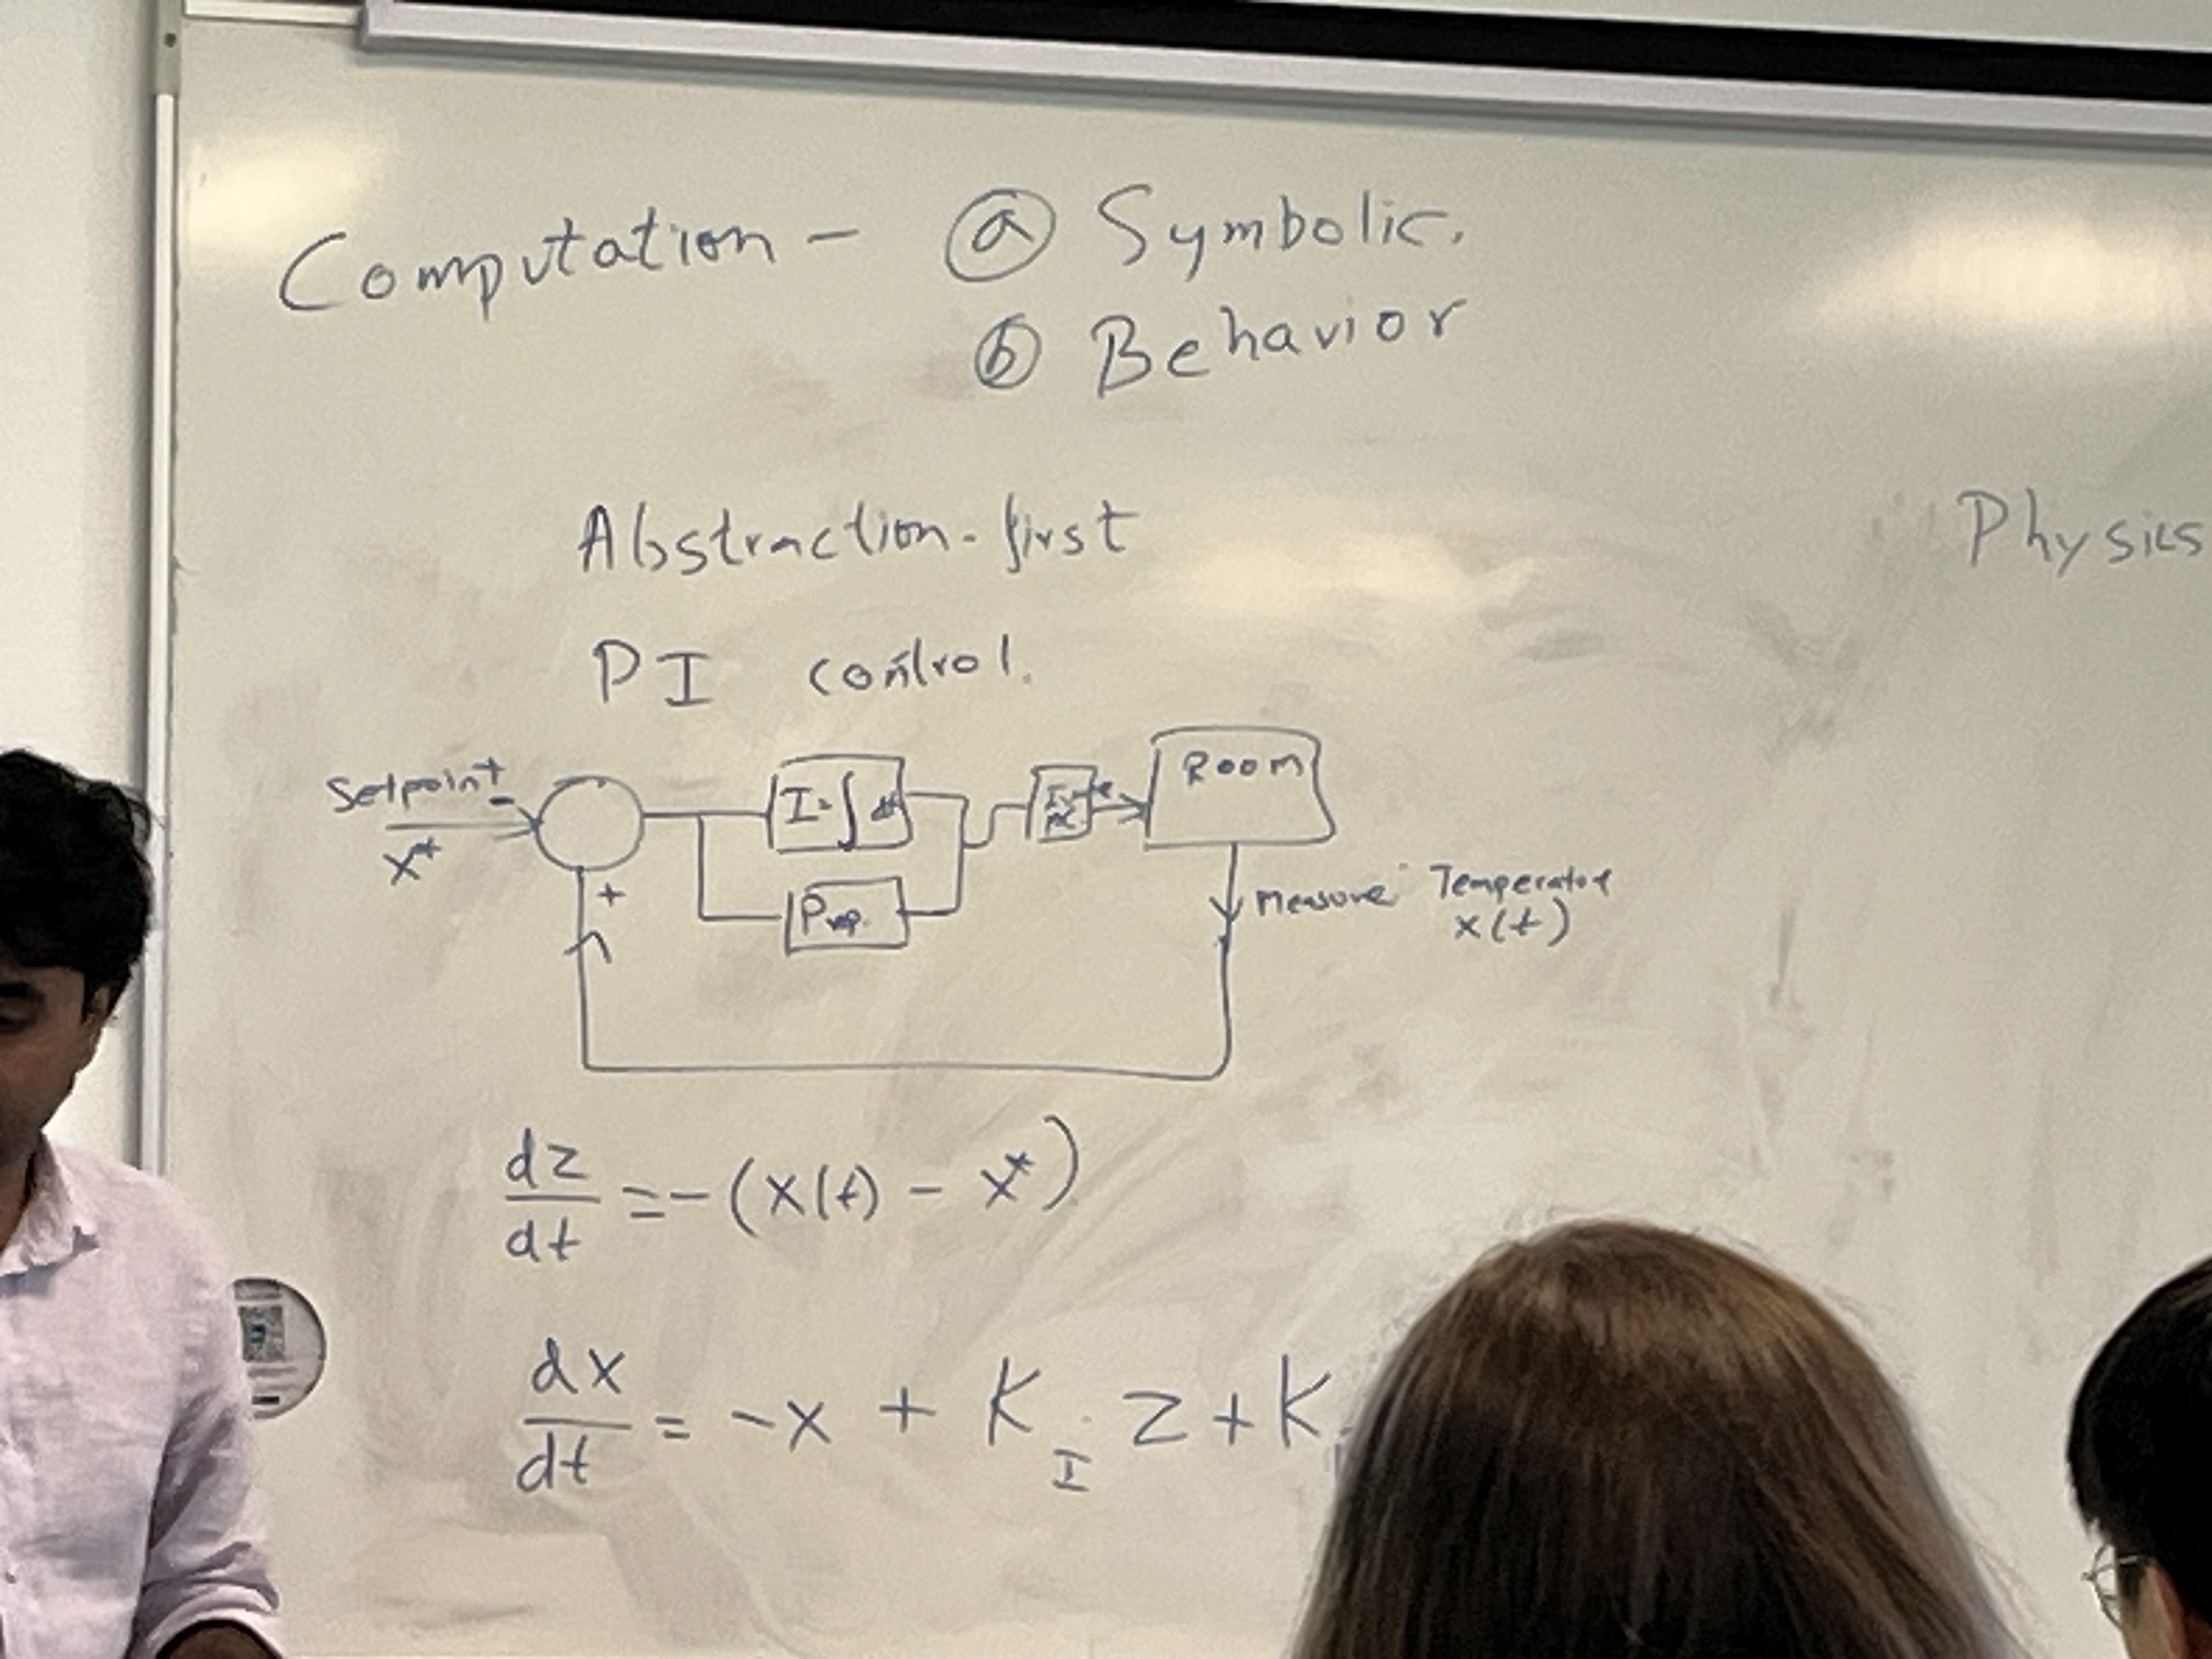
\includegraphics[scale=0.07]{figures/murugan/PI_Control.jpg}
		\caption{Diagram of control line}
	\end{figure*}\\
	This defines a differentiation equation which defines your control line $z$ due to observation of a process $x$
	\begin{itemize}
		\item Pros:
			\item General / modular
		\item Cons
			\item Cannot exploit specific physics
			\item The translation between theory vs implementation is non-trivial.
	\end{itemize}
	
	\item Physics First: 
	
	You can set up a thermodynamic state equation, and solve for the phase diagram.
	Pros and Cons
	\begin{itemize}
		\item Pros: 
			\item Fewer parts (measurement, computation), which means its more robust
			\item It's passive, meaning it self computes
		\item Cons
			\item Specific to the physics
	\end{itemize}
\end{enumerate}
This talk will focus on how to move toward the 2nd way of thinking. An example of this is the Liquid-Liquid phase transition of two liquids inside of a cell (see Zechnor 2020). You can think of this as oil and water separating.
\\
\\
There are two communities working on this
\begin{enumerate}
	\item Energy efficient computations (vs silicon). 
	\begin{itemize}
		\item Example. We currently run computations on a silicon chip, however this is not energy efficient, so much so governments are thinking about building more nuclear reactors to power the next generation of AI). So perhaps we can build biological circuits which run these computations natively on some bio-efficient chip.
		\item Example. Encode your optimization problem onto a Ising-like physical system, and anneal that system! Now you can read off optimized parameters.
		\item Example. You can use optimal computing to make better matrix multiplication.
	\end{itemize}
	\item Biological computations
	\begin{itemize}
		\item Backprop. That is each organism is reacting and adjusting it's behavior. Much more complex than just physics or chemical behavior.
		\item Evolution. No one organism does the computation, but rather it's the ensemble of them which can perform computations.
		\item Physics / Chemistry. It's just a reaction based on laws of physics / chemistry.
	\end{itemize}
\end{enumerate}
Now, how does this all relate to machine learning. Let's consider a high dimensional classifier-- you could think of the decision boundary as phase boundaries. You can also go one step further and use the transition between phases as the classifier (see \url{https://www.jbc.org/article/S0021-9258(20)36794-6/pdf} for more details)! So your features correspond to temperature, pressure, etc., and your classification is the phase. 
\begin{figure*}[h!]
	\centering
	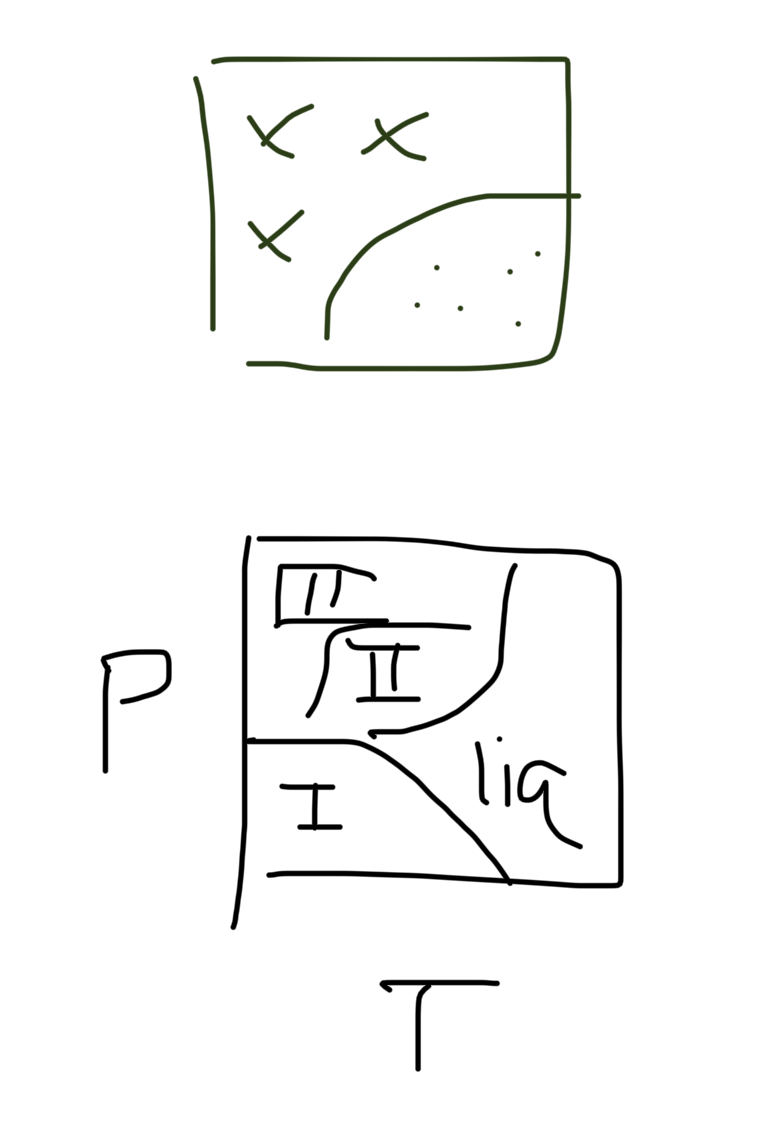
\includegraphics[scale=0.5]{figures/murugan/DecisionBoundary_PhaseDiagram.png}
	\caption{Decision boundary problems can be mapped into a physics system by inspecting their phase transition}
\end{figure*}
So the questions become what in the material / organism do I have to tune s.t. you can learn, and this also may find new interesting physical mechanisms for scientists to play with.

\subsection{Training Molecules}
\subsubsection{Hopefield Associative Memory}
Consider a set of neurons $\{x_i\}^N_{i=1}$ which take on binary values $x_i \in \{\pm 1\}$.  It takes on discrete dyanmics
\begin{align}
	x_i(t+1) = \text{sign}\left(\sum_j J_{ij} x_j(t) + h_i^{ext}(t) 
\right)
\end{align}
Your task is a supervised learning problem... The goal is to store a set of memories $m_i^\alpha \in \mathbb R^N$ (s.t. $\alpha = 1,..., M$). And you want to retrieve a memory $m$ from a just showing a partial part of $m$ (association). That is you want your neurons $\{x_i\}$ to fire in the same pattern as $m$ \\
\\
To train this model, we use a \textbf{Hebbian} learning rule
\begin{align}
	\frac{dJ_{ij}}{dt} = x_i (t) x_j(t)
\end{align}
We run this every time we should it a new memory. So for example, after being exposed to 3 memories $\{m^{(1)}, m^{(2)}, m^{(3)}\}$, our couplings look like $J_{ij} = m_i^{(1)} m_j^{(1)} + m_i^{(2)} m_j^{(2)} + m_i^{(3)} m_j^{(3)}$. Running this process will make the energy landscape become low where $x = m^{(i)}$-- so if you train on images, and then show noised versions of those images, then you'll be-able to denoise said images! Very cool! 

Note that hopfield networks have a memory capacity $M_c$, so this only works when the total memories $M < M_c$.

\subsubsection{Multifavious Assembly Mixtures}
Here we'll consider a physical system which is analogous to Hopfield's Assocative Memory model.

Consider $N$ molecular species in a solvent (this is different from the number of molecules, for example these can be $N$ proteins with different names), with binding interactions $J_{ij}$, and concentrations $C_i(x,t)$ at position $x$ at time $t$ (and associated chemical potentials $\mu_i$). The molecules are held at a physical temperature $T$, and have diffusion constant $D_i$.

\begin{align}
	\frac{dJ_{ij}}{dt} = - \int d^3x ~dt ~ C_i(x,t) C_j(x,t)
\end{align}
This rule says, these molecules will increase their bond ($J_{ij}$ will increase) if there are more of said molecules in the same place ($C_i(x,t) C_j(x,t)$ is the concentrations of molecules $i$ and $j$ at position $x$ at time $t$).

In practice, we need to use \textbf{linkers} (these are other molecules which mediate interactions between molecules). So they can be used to tune your $J_{ij}$'s.

The associative memory is to reconstruct a set of protein binded together. So you can construct a memory as a sequence of proteins, cut it up, place it into the test tube, and see if it can reconstruct the previous protein.


















\newpage




\newpage

\part{Other Things}

\section{People Presentations} 
\begin{enumerate}
	\item Paolo Balioni, working on feature learning in Bayesian Neural Networks. Also works on MCMC methods.
	\item Claudian Merger. Mappping normalizing flows to $\phi^n$ theory.
\end{enumerate}



\end{document}